\documentclass[tikz, border=10pt]{standalone}
\usepackage{tikz}

\begin{document}
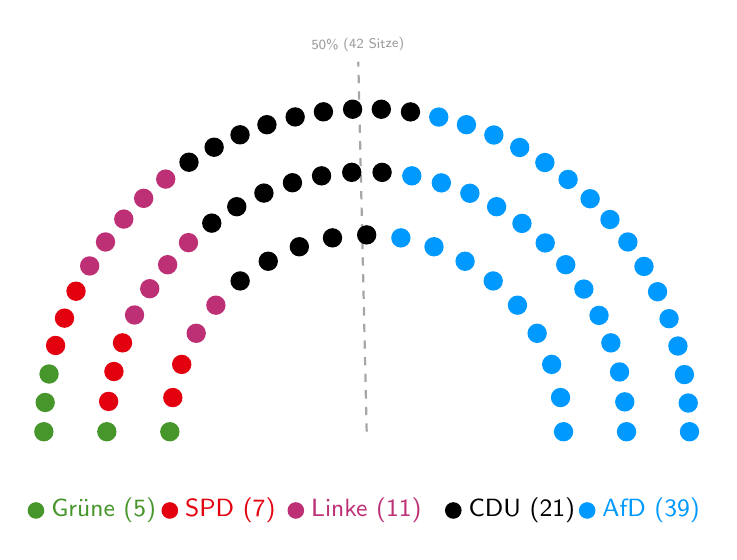
\begin{tikzpicture}

% Define Party Colors
\definecolor{AfDColor}{HTML}{0099FF}
\definecolor{CDUColor}{HTML}{000000}
\definecolor{LinkeColor}{HTML}{BE3075}
\definecolor{SPDColor}{HTML}{E3000F}
\definecolor{GrueneColor}{HTML}{46962B}

\begin{scope}[scale=1]

  % 50% Majority Divider Line & Annotation
  % 83 total seats -> 50% majority threshold = 42 seats
  % The 42nd seat counter-clockwise sits near ~91.3 degrees
  \draw[dashed, thick, gray!70] (0,0) -- (91.3:4.7cm);
  \node[font=\tiny\sffamily, color=gray!80, rotate=1.3, anchor=south] at (91.3:4.7cm) {50\% (42 Sitze)};

  % Arc 1 (Inner Row - 19 Seats)
  \foreach \angle/\col in {
    0/AfDColor, 10/AfDColor, 20/AfDColor, 30/AfDColor, 40/AfDColor, 50/AfDColor, 60/AfDColor, 70/AfDColor, 80/AfDColor,
    90/CDUColor, 100/CDUColor, 110/CDUColor, 120/CDUColor, 130/CDUColor,
    140/LinkeColor, 150/LinkeColor,
    160/SPDColor, 170/SPDColor, 180/GrueneColor%
  } {
    \fill[\col] (\angle:2.5cm) circle (3.5pt);
  }

  % Arc 2 (Middle Row - 28 Seats)
  \foreach \angle/\col in {
    0/AfDColor, 6.6/AfDColor, 13.3/AfDColor, 20/AfDColor, 26.6/AfDColor, 33.3/AfDColor, 40/AfDColor, 46.6/AfDColor, 53.3/AfDColor, 60/AfDColor, 66.6/AfDColor, 73.3/AfDColor, 80/AfDColor,
    86.6/CDUColor, 93.3/CDUColor, 100/CDUColor, 106.6/CDUColor, 113.3/CDUColor, 120/CDUColor, 126.6/CDUColor,
    133.3/LinkeColor, 140/LinkeColor, 146.6/LinkeColor, 153.3/LinkeColor,
    160/SPDColor, 166.6/SPDColor, 173.3/SPDColor, 180/GrueneColor%
  } {
    \fill[\col] (\angle:3.3cm) circle (3.5pt);
  }

  % Arc 3 (Outer Row - 36 Seats)
  \foreach \angle/\col in {
    0/AfDColor, 5.1/AfDColor, 10.2/AfDColor, 15.4/AfDColor, 20.5/AfDColor, 25.7/AfDColor, 30.8/AfDColor, 36/AfDColor, 41.1/AfDColor, 46.2/AfDColor, 51.4/AfDColor, 56.5/AfDColor, 61.7/AfDColor, 66.8/AfDColor, 72/AfDColor, 77.1/AfDColor,
    82.2/CDUColor, 87.4/CDUColor, 92.5/CDUColor, 97.7/CDUColor, 102.8/CDUColor, 108/CDUColor, 113.1/CDUColor, 118.2/CDUColor, 123.4/CDUColor,
    128.5/LinkeColor, 133.7/LinkeColor, 138.8/LinkeColor, 144/LinkeColor, 149.1/LinkeColor,
    154.2/SPDColor, 159.4/SPDColor, 164.5/SPDColor,
    169.7/GrueneColor, 174.8/GrueneColor, 180/GrueneColor%
  } {
    \fill[\col] (\angle:4.1cm) circle (3.5pt);
  }

\end{scope}

% Legend (Ordered Left-to-Right: Grüne, SPD, Die Linke, CDU, AfD)
\begin{scope}[shift={(0,-1.0)}]
  \fill[GrueneColor] (-4.2, 0) circle (3pt) node[right=2pt, font=\small\sffamily] {Grüne (5)};
  \fill[SPDColor] (-2.5, 0) circle (3pt) node[right=2pt, font=\small\sffamily] {SPD (7)};
  \fill[LinkeColor] (-0.9, 0) circle (3pt) node[right=2pt, font=\small\sffamily] {Linke (11)};
  \fill[CDUColor] (1.1, 0) circle (3pt) node[right=2pt, font=\small\sffamily] {CDU (21)};
  \fill[AfDColor] (2.8, 0) circle (3pt) node[right=2pt, font=\small\sffamily] {AfD (39)};
\end{scope}

\end{tikzpicture}
\end{document}